\documentclass[a4paper]{article}

%% Language and font encodings
\usepackage[english]{babel}
\usepackage[utf8x]{inputenc}
\usepackage[T1]{fontenc}

%% Sets page size and margins
\usepackage[a4paper,top=3cm,bottom=2cm,left=3cm,right=3cm,marginparwidth=1.75cm]{geometry}

%% Useful packages
\usepackage{amsmath}
\usepackage{graphicx}
\usepackage[colorinlistoftodos]{todonotes}
\usepackage[colorlinks=true, allcolors=blue]{hyperref}

\title{Documentation - PreDeCon Algorithm }
\author{Group 3: Brandl Moritz, Miklautz Lukas, Mitsch Raphael}

\begin{document}
\maketitle


\section{Introduction}
In this paper the PreDeCon (subspace PREference weighted DEnsity and CONnected clustering) algorithm is explained. The algorithm was created by B\"ohm, Christian, et al.\cite{bohm2004density}  in 2004. PreDeCon  is a clustering algorithm that was developed to perform well in high-dimensional feature spaces. High-dimensional feature spaces cause many clustering algorithms to break down, due to the curse of dimensionality. In this case this refers to the phenomenon, that clustering algorithms which calculate  distances in the full dimensional space deteriorate in performance, because the distances in such spaces lose their meaning. That's why specialized clustering algorithms were developed, which are based on the observation that clusters exist only in specific subspaces of the full feature space. There are several approaches to this problem, two of them will be explained here briefly. Subspace clustering tries to find all possible clusters in all axis-parallel subspaces in a bottom-up way, here it is possible for clusters to overlap, this means that points can be assigned to multiple clusters, see \cite{agrawal1998automatic} and \cite{kailing2004density}. In projected clustering all points are uniquely assigned to clusters or noise in a top-down approach, therefor clusters cannot overlap. 

\section{The PreDeCon Algorithm}
PreDeCon belongs to the group of projected clustering algorithms. It follows an instance-based approach, which calculates for each point in the data base a subspace preference in the entire feature space and merges the points with similar preferences together to form a cluster. 
The rational behind this approach follows the locality assumption, which states that "the subspace preference can be learned from the local neighborhood in the d-dimensional space", as mentioned in the courses slides.
PreDeCon is based on the density-based clustering algorithm DBSCAN \cite{ester1996density} and can be seen as an extension of it for high-dimensional spaces. 
PreDeCon has the following features\cite{bohm2004density}:
\begin{itemize}
\item the clustering result is determinate
\item it is robust against noise
\item it has a worst-case time complexity of $O(dn^2)$
\end{itemize}


\subsection{Underlying Ideas}
The underlying idea of PreDecon is the "subspace preference cluster" \cite{bohm2004density}, which expands the idea of density connected set of points by a subspace preference vector. Note, that from now on all points $p,q$ are considered as elements of the data base. The subspace preference vector skews the  $\epsilon$-neighborhood of point $p$ in the direction of the lowest attribute variance, where the attribute variance of a point $p$ is given by: 
$$VAR_{A_i}(N_{\epsilon}(p))=\frac {\sum_{q \in (N_{\epsilon}(p))} (dist(\pi_{A_i}(p),\pi_{A_i}(q)))^2} {|N_{\epsilon}(p)|}$$
From the attribute variance the subspace preference vector of a point p is derived as
\[ w_i =
  \begin{cases}
    1       & \quad \text{if } VAR_{A_i}(N_{\epsilon}(p))  > \delta \\
    \kappa  & \quad \text{if } VAR_{A_i}(N_{\epsilon}(p))  \leq \delta
  \end{cases}
\]
and the preference weighted similarity measure associated with a point p can then be calculated as a simple weighted Euclidean distance \cite{bohm2004density}. Here the parameter $\delta$ specifies the threshold for a low variance. Due to the weighting factor this similarity measure is asymmetric, this means that $dist_{p}(p,q) = dist_{p}(q,p)$ does not hold anymore. This can be corrected by using the maximum of the two distances, see \cite{bohm2004density}. Look at figure \ref{fig:predecon_epsilon_neighbourhood}, to see the consequences of the preference weighted Euclidean distance. With this new weighted distance function the preference weighted $\epsilon$-neighborhood for each point can be calculated. Another important concept which has been adapted from DBSCAN are the preference weighted core points. Similar to the definition of core points in DBSCAN a preference weighted core point needs to have a minimum number of points in its preference weighted $\epsilon$-neighborhood, denoted by the parameter $\mu$. The PreDeCon algorithm allows the user to specify additionally a maximum preference dimensionality of the $\epsilon$-neighbourhood of a point, denoted as $\lambda$. The last notion in order for PreDeCon to work is the direct preference weighted reachability. It states that a point $p$ is direct preference weighted reachable from a point $q$ if $q$ is a preference weighted core point, the preference weighted dimensionality of the $\epsilon$-neighborhood of point p is smaller or equal to $\lambda$ and p is in the preference weighted epsilon neighborhood of q. For a more detailed explanation of these concepts refer to \cite{bohm2004density}.

\begin{figure}
\centering
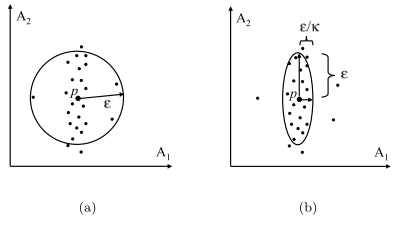
\includegraphics[width=0.6\textwidth]{predecon_epsilon_neighbourhood.PNG}
\caption{ $\epsilon$-neighborhood of p according to (a) simple
Euclidean and (b) preference weighted Euclidean distance.(Figure taken from \cite{bohm2004density})}
\label{fig:predecon_epsilon_neighbourhood}
\end{figure}

\begin{figure}
\centering
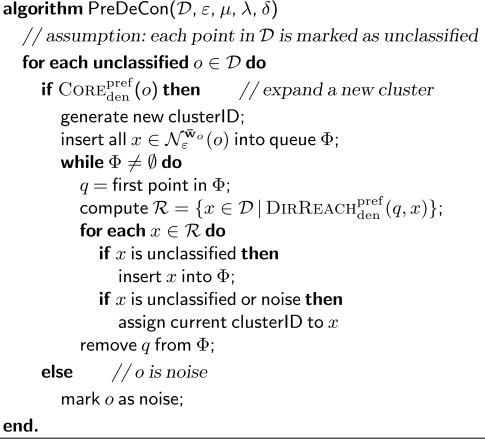
\includegraphics[width=0.6\textwidth]{predecon_pseudocode_paper.PNG}
\caption{Pseudo code of the PreDeCon algorithm.(Figure taken from \cite{bohm2004density})}
\label{fig:pseudocode_paper}
\end{figure}

\subsection{The Algorithm}
PreDeCon needs the following user specified parameters\cite{bohm2004density}:
\begin{itemize}
\item $\mu$: Minimal number of points in $\epsilon$-neighborhood
\item $\epsilon$: Distance parameter for neighborhood calculation
\item $\delta$: Variance threshold for subspace preference clusters
\item $\lambda$: Threshold for dimensionality of $\epsilon$-neighbourhood of a point
\item $\kappa$: Weight for subspace preference vectors
\end{itemize}

In figure \ref{fig:pseudocode_paper} the pseudo code of the original paper is shown. The inner workings of this algorithm are explained in the next section, when the implementation of PreDeCon are discussed.



\section{The Pseudocode of our implementation}
Enter pseudocode of our implementation as soon as finished.
\section{Parameter Tuning}
To compare and benchmark our algorithm we took the "Vary Density" data set from the Elki homepage.
In order to find a suitable tuple of parameters, we first tried guessing a somewhat good combination of parameters and then do a grid search around those parameters to find the best combination. Therefore we first came up with following parameters as shown in Figure \ref{fig:init_paramt}:
\begin{enumerate}
\item epsilon: 0.3
\item mu: 10
\item delta: 0.1
\item kappa: 20
\item lambda: 2
\end{enumerate}

\begin{figure}
	\centering
	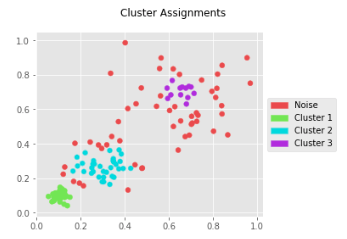
\includegraphics[width=0.6\textwidth]{init_paramt.png}
	\caption{Result of PreDeCon-algorithm with initial parameters}
    \label{fig:init_paramt}
\end{figure}

By feeding the same parameter combination into elki we obtain the same clusters, shown in Figure \ref{fig:elki_init_paramt}

\begin{figure}
	\centering
	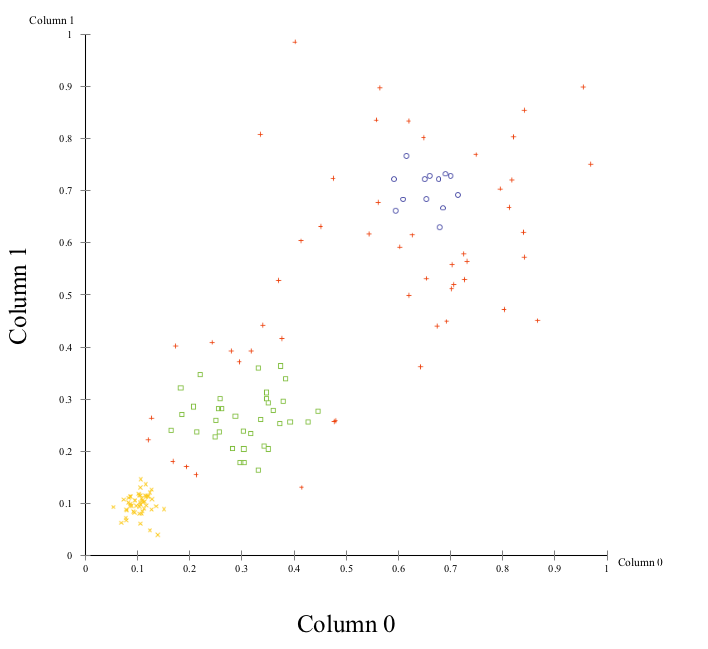
\includegraphics[width=0.6\textwidth]{elki_init_paramt.png}
	\caption{ Result of PreDeCon-algorithm in ELKI with initial parameters}
    \label{fig:elki_init_paramt}
\end{figure}
\paragraph{}
We then applied two different clustering performance evaluation methods onto the several models we calculated. We used Adjusted-Normalized-Information (AMI) and also V-Measure. Both measurements resulted in different "best" parameter combinations. While the AMI chose our initial parameter settings to be the best (Figure \ref{fig:ami_dict}), the V-Measurement chose a completely different model. (Figure \ref{fig:v_score_dict}). 

\begin{figure}
	\label{fig:ami_dict}
	\centering
	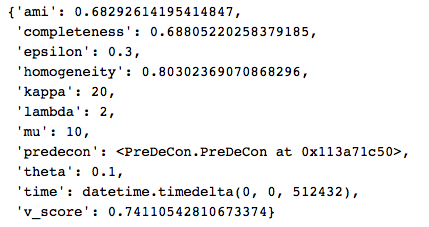
\includegraphics[width=0.6\textwidth]{ami_dict.png}
	\caption{Best result when looking at adjusted mutual information}
\end{figure}

\begin{figure}
	\centering
	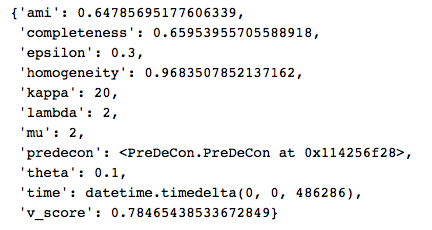
\includegraphics[width=0.6\textwidth]{v_score_dict.png}
	\caption{Best result when looking at v score}
    \label{fig:v_score_dict}
\end{figure}

\begin{figure}
	\centering
	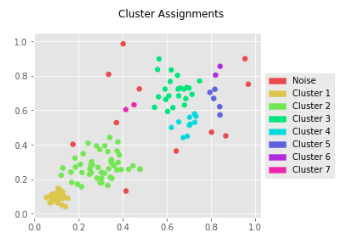
\includegraphics[width=0.6\textwidth]{v_score_graph.png}
	\caption{Clustering when choosing parameters of v-score winner}
    \label{fig:v_score_graph}
\end{figure}
\paragraph{}
When looking at Figure \ref{fig:v_score_graph} we can see that according to the V-Measurement the best score is achieved by 7 clusters. In addition to the v-score we also have the completeness and homogeneity measures which both are actually used to calculated the v-score. by definition, the homogeneity measures if each cluster contains only members of a single class. We achieved a homogeneity of 0.9683 as can be seen in Figure \ref{fig:v_score_dict}. In the original data set, there are only 3 clusters and no noise points. In this clustering, the few noise points which are basically assigned to the cluster "noise" come from different ground-truth clusters. every other cluster is within only one of the ground-truth clusters. therefore this score is almost 1. On the other hand completeness is defined as: all members of a given class are assigned to the same cluster. as there are more than 3 clusters, this cannot be true, so this is why this score is at 0.6595 (see Figure \ref{fig:v_score_dict}).

\section{Benchmarking}
We can already see that the clustering of both the PreDeCon implementation in elki as well as our own have the same result. Though, when it comes to runtime we are far worse off than elki. Elki needs about 6ms to finish the clustering of Figure \ref{fig:v_score_dict}, while our algorithm needs 486ms.

\bibliographystyle{alpha}
\bibliography{sample}

\end{document}